\documentclass[a4paper, 12pt]{article}
\usepackage{ctex} % 支持中文
\usepackage{geometry} % 设置页边距
\usepackage{graphicx} % 支持插入图片
\usepackage{booktabs} % 支持三线表
\usepackage{float} % 控制图表位置
\usepackage{titlesec} % 自定义标题格式
\pagestyle{empty}      % 去掉页眉页脚
\usepackage{float}      % 用于强制图片位置


\geometry{a4paper, left=3cm, right=3cm, top=2.5cm, bottom=2.5cm}


% \renewcommand{\thesection}{\chinese{section}、} % 将section编号改为 "一、", "二、"
\titleformat{\section}{\Large\bfseries\centering}{\thesection}{1em}{} % 设置格式为居中、黑体


\pagestyle{empty}

\begin{document}

% 封面
\begin{titlepage}
    \centering
    \vspace*{\stretch{1.0}}
    
    {\Huge\heiti 西安理工大学}
    \vspace{1.5cm}
    
    {\fontsize{22}{26}\selectfont\heiti 智能传感与测试技术 B}
    \vspace{0.8cm}
    
    {\fontsize{22}{26}\selectfont\heiti 实践作业}
    \vspace{\stretch{2.0}}
    
    \large
    \begin{tabular}{@{}l@{\hspace{1em}}l@{}}
        \textbf{班\quad 级：} & \underline{\hspace{2em}工业工程 232 班\hspace{5cm}} \\
        \addlinespace[1.5em]
        \textbf{任课教师：} & \underline{\hspace{2em}郭伟超\hspace{7.5cm}} \\
        \addlinespace[1.5em]
        \textbf{姓\quad 名：} & \underline{\hspace{2em}安家乐~~~闫小杰\hspace{6cm}} \\
        \addlinespace[1.5em]
        \textbf{成\quad 绩：} & \underline{\hspace{10cm}} \\
        \addlinespace[1.5em]
        \textbf{完成时间：} & \underline{\hspace{2em}2025 年 10 月 12 日\hspace{4cm}} \\
    \end{tabular}
    
    \vspace{\stretch{1.0}}
\end{titlepage}



\section{应用场景}


在传统的仓储管理模式中，物料信息的采集主要依赖于人工手持扫描枪对一维或二维条码进行逐一扫描。这种模式在高密度、高通量的现代化仓储作业中暴露了诸多问题：

\begin{enumerate}
    \item \textbf{入库效率低下}：货物送达后，需要人工开箱，并对箱内每一件商品进行扫描，以核对数量和信息，整个过程耗时耗力，容易在入库环节形成拥堵。对于一个包含上千件商品的托盘，传统扫描方式可能需要数十分钟甚至更长时间。
    \item \textbf{出库复核易出错}：拣货完成后，同样需要人工逐一扫描复核，以确保出库的商品与订单完全一致。在高强度的作业压力下，人工操作极易出现漏扫或错扫，导致发货错误，引发客户投诉和经济损失。
    \item \textbf{库存盘点难度大}：传统的盘点工作需要中断正常的仓储作业，由工作人员对货架上的商品进行逐件清点和扫描，不仅工作量巨大，耗时漫长，而且难以保证数据的绝对准确。一次全仓盘点往往需要数天时间，期间无法进行正常的出入库作业，影响企业运营。
\end{enumerate}

为解决上述痛点，引入以射频识别（Radio Frequency Identification, RFID）技术为核心的智能传感系统，旨在利用其非接触、批量读取的特性，实现物料信息的自动化、高效率采集，从而彻底变革仓储作业流程，提升整体管理水平与运营效率 \cite{ref1}。

\section{主要结构和工作原理}

\subsection{系统主要结构}

从智能传感与测试技术的角度看，RFID物料管理系统的核心是一种非接触式射频识别传感系统。其基本结构围绕着“感知-传输-处理”这一主线构建（如 \figurename~\ref{fig:system_structure} 所示）：

\begin{figure}[H]
    \centering
    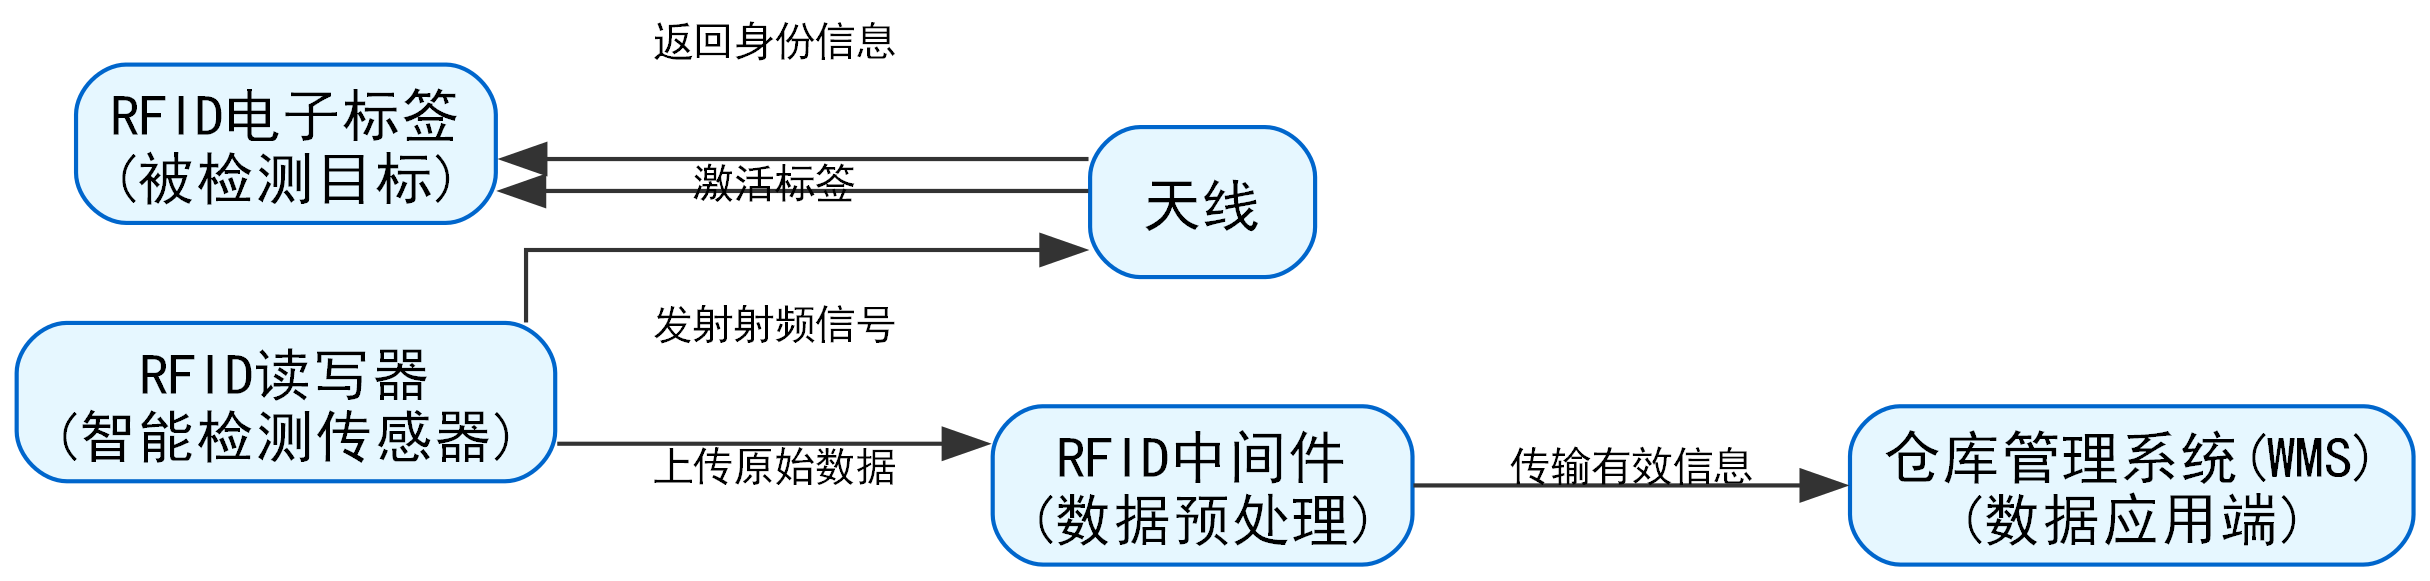
\includegraphics[width=14cm,height=3.5cm]{system_structure.png}
    \caption{RFID系统结构示意图}
    \label{fig:system_structure}
\end{figure}


\begin{itemize}
    \item \textbf{核心传感单元}：
    \begin{itemize}
        \item \textbf{RFID读写器 (Reader)}：作为主要的智能检测传感器，它内部集成了射频模块、控制单元和通信接口，不仅能主动发射特定频率的电磁波以“探寻”目标，还能接收并解码从目标返回的微弱信号。其“智能”体现在它能够根据指令控制发射功率、选择特定通道，并能对采集到的信号进行初步处理和校验。
    \end{itemize}
    \item \textbf{被检测目标/信号源}：
    \begin{itemize}
        \item \textbf{RFID电子标签 (Tag)}：作为依附在被测物料上的“信号源”。它内部含有天线和微型芯片，芯片中存储了物料的唯一身份信息\cite{ref2}。当它进入读写器（传感器）的电磁场范围时，会被激活并将自身信息编码后发射出去。
    \end{itemize}
    \item \textbf{传感信号的辅助单元}：
    \begin{itemize}
        \item \textbf{天线 (Antenna)}：作为读写器传感器的一部分，是其“感知”范围的延伸。它负责将读写器的电信号转换成空间传播的电磁波，并发射出去；同时，也负责捕获标签返回的微弱电磁波，并将其转换成电信号送回读写器进行处理。
    \end{itemize}
    \item \textbf{数据处理与应用单元}：
    \begin{itemize}
        \item \textbf{RFID中间件 (Middleware)}：可以看作是传感器的“驱动程序”和“数据预处理器”。它负责管理和控制一个或多个RFID读写器，并对传感器采集到的大量原始数据进行过滤、清洗和整理，最终将有价值的信息流传送给上层应用。
        \item \textbf{仓库管理系统 (WMS)}：这是传感器数据的最终应用端。它接收、存储并利用传感器提供的实时物料数据，实现库存管理、作业调度等业务逻辑。
    \end{itemize}
\end{itemize}




为了更清晰地展示系统构成，\tablename~\ref{tab:equipment_list} 列出了本案例中RFID系统的主要设备。


\begin{table}[H]
    \centering
    \setlength{\belowcaptionskip}{0.3cm}
    \caption{RFID系统主要设备列表}
    \label{tab:equipment_list}
    \begin{tabular}{c c c}
        \toprule
        \textbf{序号} & \textbf{名称} & \textbf{功能说明} \\
        \midrule
        1 & 固定式RFID读写器 & 安装在出入库通道，用于自动、批量采集货物信息 \\
        2 & 手持式RFID读写器 & 用于移动盘点和货物查找 \\
        3 & RFID电子标签 & 粘贴于货箱或单品上，存储唯一标识信息 \\
        4 & RFID中间件服务器 & 负责管理读写器，并对采集的原始数据进行处理 \\
        5 & 仓库管理系统(WMS) & 接收处理后的数据，进行库存更新和业务管理 \\
        \bottomrule
    \end{tabular}
\end{table}

\subsection{工作原理与流程}

结合应用场景，整个工作流程本质上是一系列由RFID传感器主导的自动化检测与数据采集过程，其与传统流程的对比如 \figurename~\ref{fig:workflow} 所示。

\begin{itemize}
    \item \textbf{入库自动检测}：当货物通过入库通道时，被部署在该处的固定式读写器（传感器）所覆盖。传感器主动发射射频信号，形成一个“电磁检测区域”。区域内所有货箱上的RFID标签被能量激活，做出响应。传感器通过天线阵列高速地轮询检测并捕获所有标签返回的信号，解码出其ID信息，完成对整批货物的非接触式、批量化数据采集，并将数据上传\cite{ref3}。
    \item \textbf{出库自动校验}：同理，在出库口，传感器再次对即将发出的货物进行一次全面的扫描检测。这个过程相当于对订单进行一次高速、自动化的物理校验。WMS将传感器实时采集到的货物列表与电子订单进行比对，任何差异都会触发系统报警，从而实现了零误差的智能校验。
    \item \textbf{移动盘点}：在库存盘点中，工作人员手持的移动读写器就是一个便携式的智能传感终端。工作人员通过它主动发起对指定区域货物的信号探测。读写器在短时间内即可完成对其感知范围内所有物料信息的采集，极大地提升了盘点工作的效率和精度\cite{ref4}。
\end{itemize}


\begin{figure}[H]
    \centering
    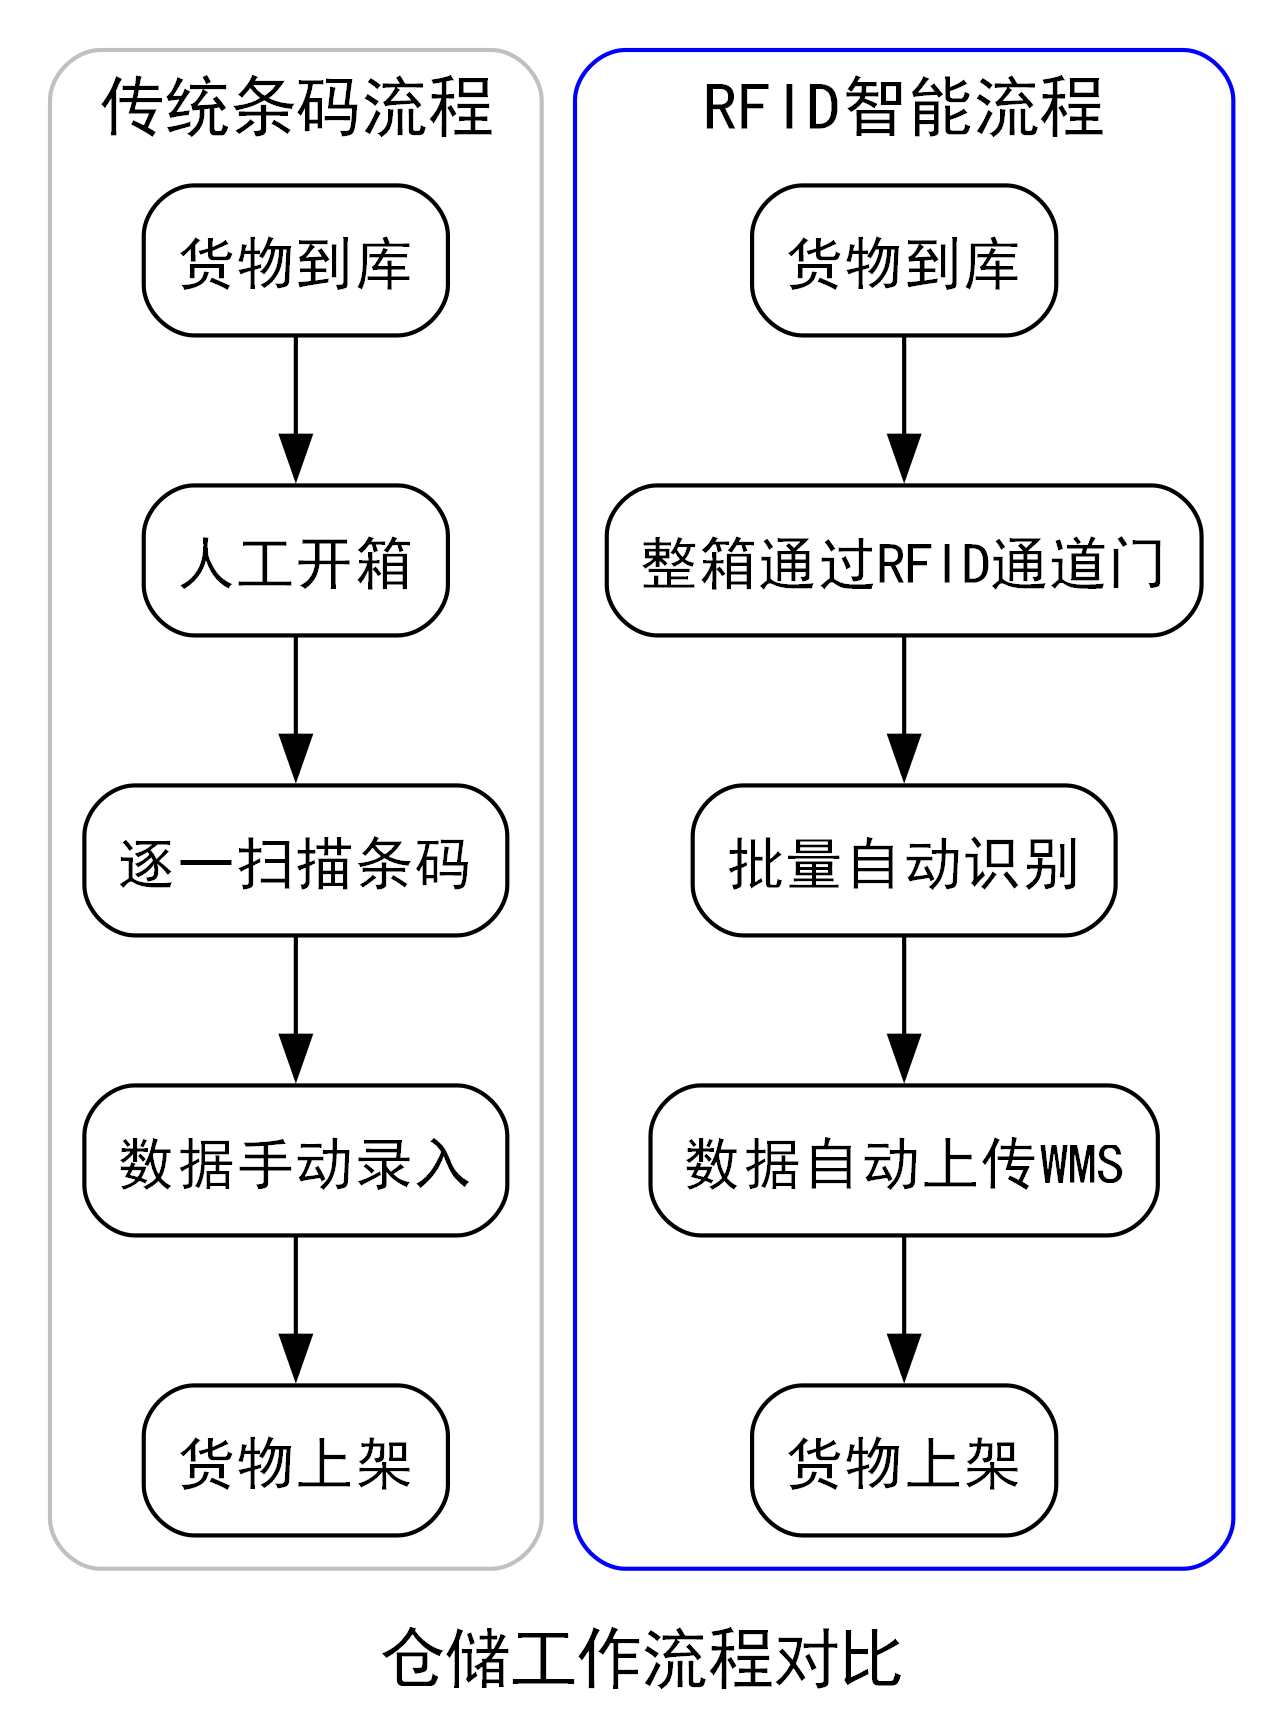
\includegraphics[width=6cm,height=8cm]{workflow_comparison.png}
    \caption{传统条码与RFID仓储工作流程对比}
    \label{fig:workflow}
\end{figure}

\subsection{优势分析与总结}

\subsubsection{技术优势分析}
如 \figurename~\ref{fig:efficiency} 所示，RFID技术的应用在多个关键绩效指标上都远超传统条码技术。
\begin{itemize}
    \item \textbf{读取便捷高效}：核心优势在于实现了非接触式、远距离、批量的快速读取。传感器无需像扫描枪一样进行精确瞄准，即可在数米范围内同时识别成百上千个标签，这使得整箱、整托盘货物的秒级数据采集成为可能，极大地提升了作业效率\cite{ref1}。
    \item \textbf{数据容量大，信息可追溯}：RFID标签芯片可存储数千字节的信息，远超传统条码的几十个字符。这不仅能记录产品的唯一ID，还能写入生产日期、批次、目的地等丰富信息。芯片数据可加密、可反复读写，为货物的全生命周期追溯和动态信息管理提供了坚实基础\cite{ref2}。
    \item \textbf{准确率高，降低人力成本}：自动化数据采集取代了重复、枯燥的人工扫描操作，从根本上避免了因视觉疲劳、操作疏忽导致的漏扫、错扫问题，将数据准确率提升至99.9\%以上，同时显著降低了对一线操作人员的依赖。
    \item \textbf{环境适应性强}：RFID标签多采用PET等材料封装，具有防水、防磁、耐高温等特性。其无线射频信号能穿透纸箱、塑料等非金属包装，即使标签表面有污损或被遮挡，传感器依然能准确读取，比易污损的光学条码更可靠。
\end{itemize}


\begin{figure}[H]
    \centering
    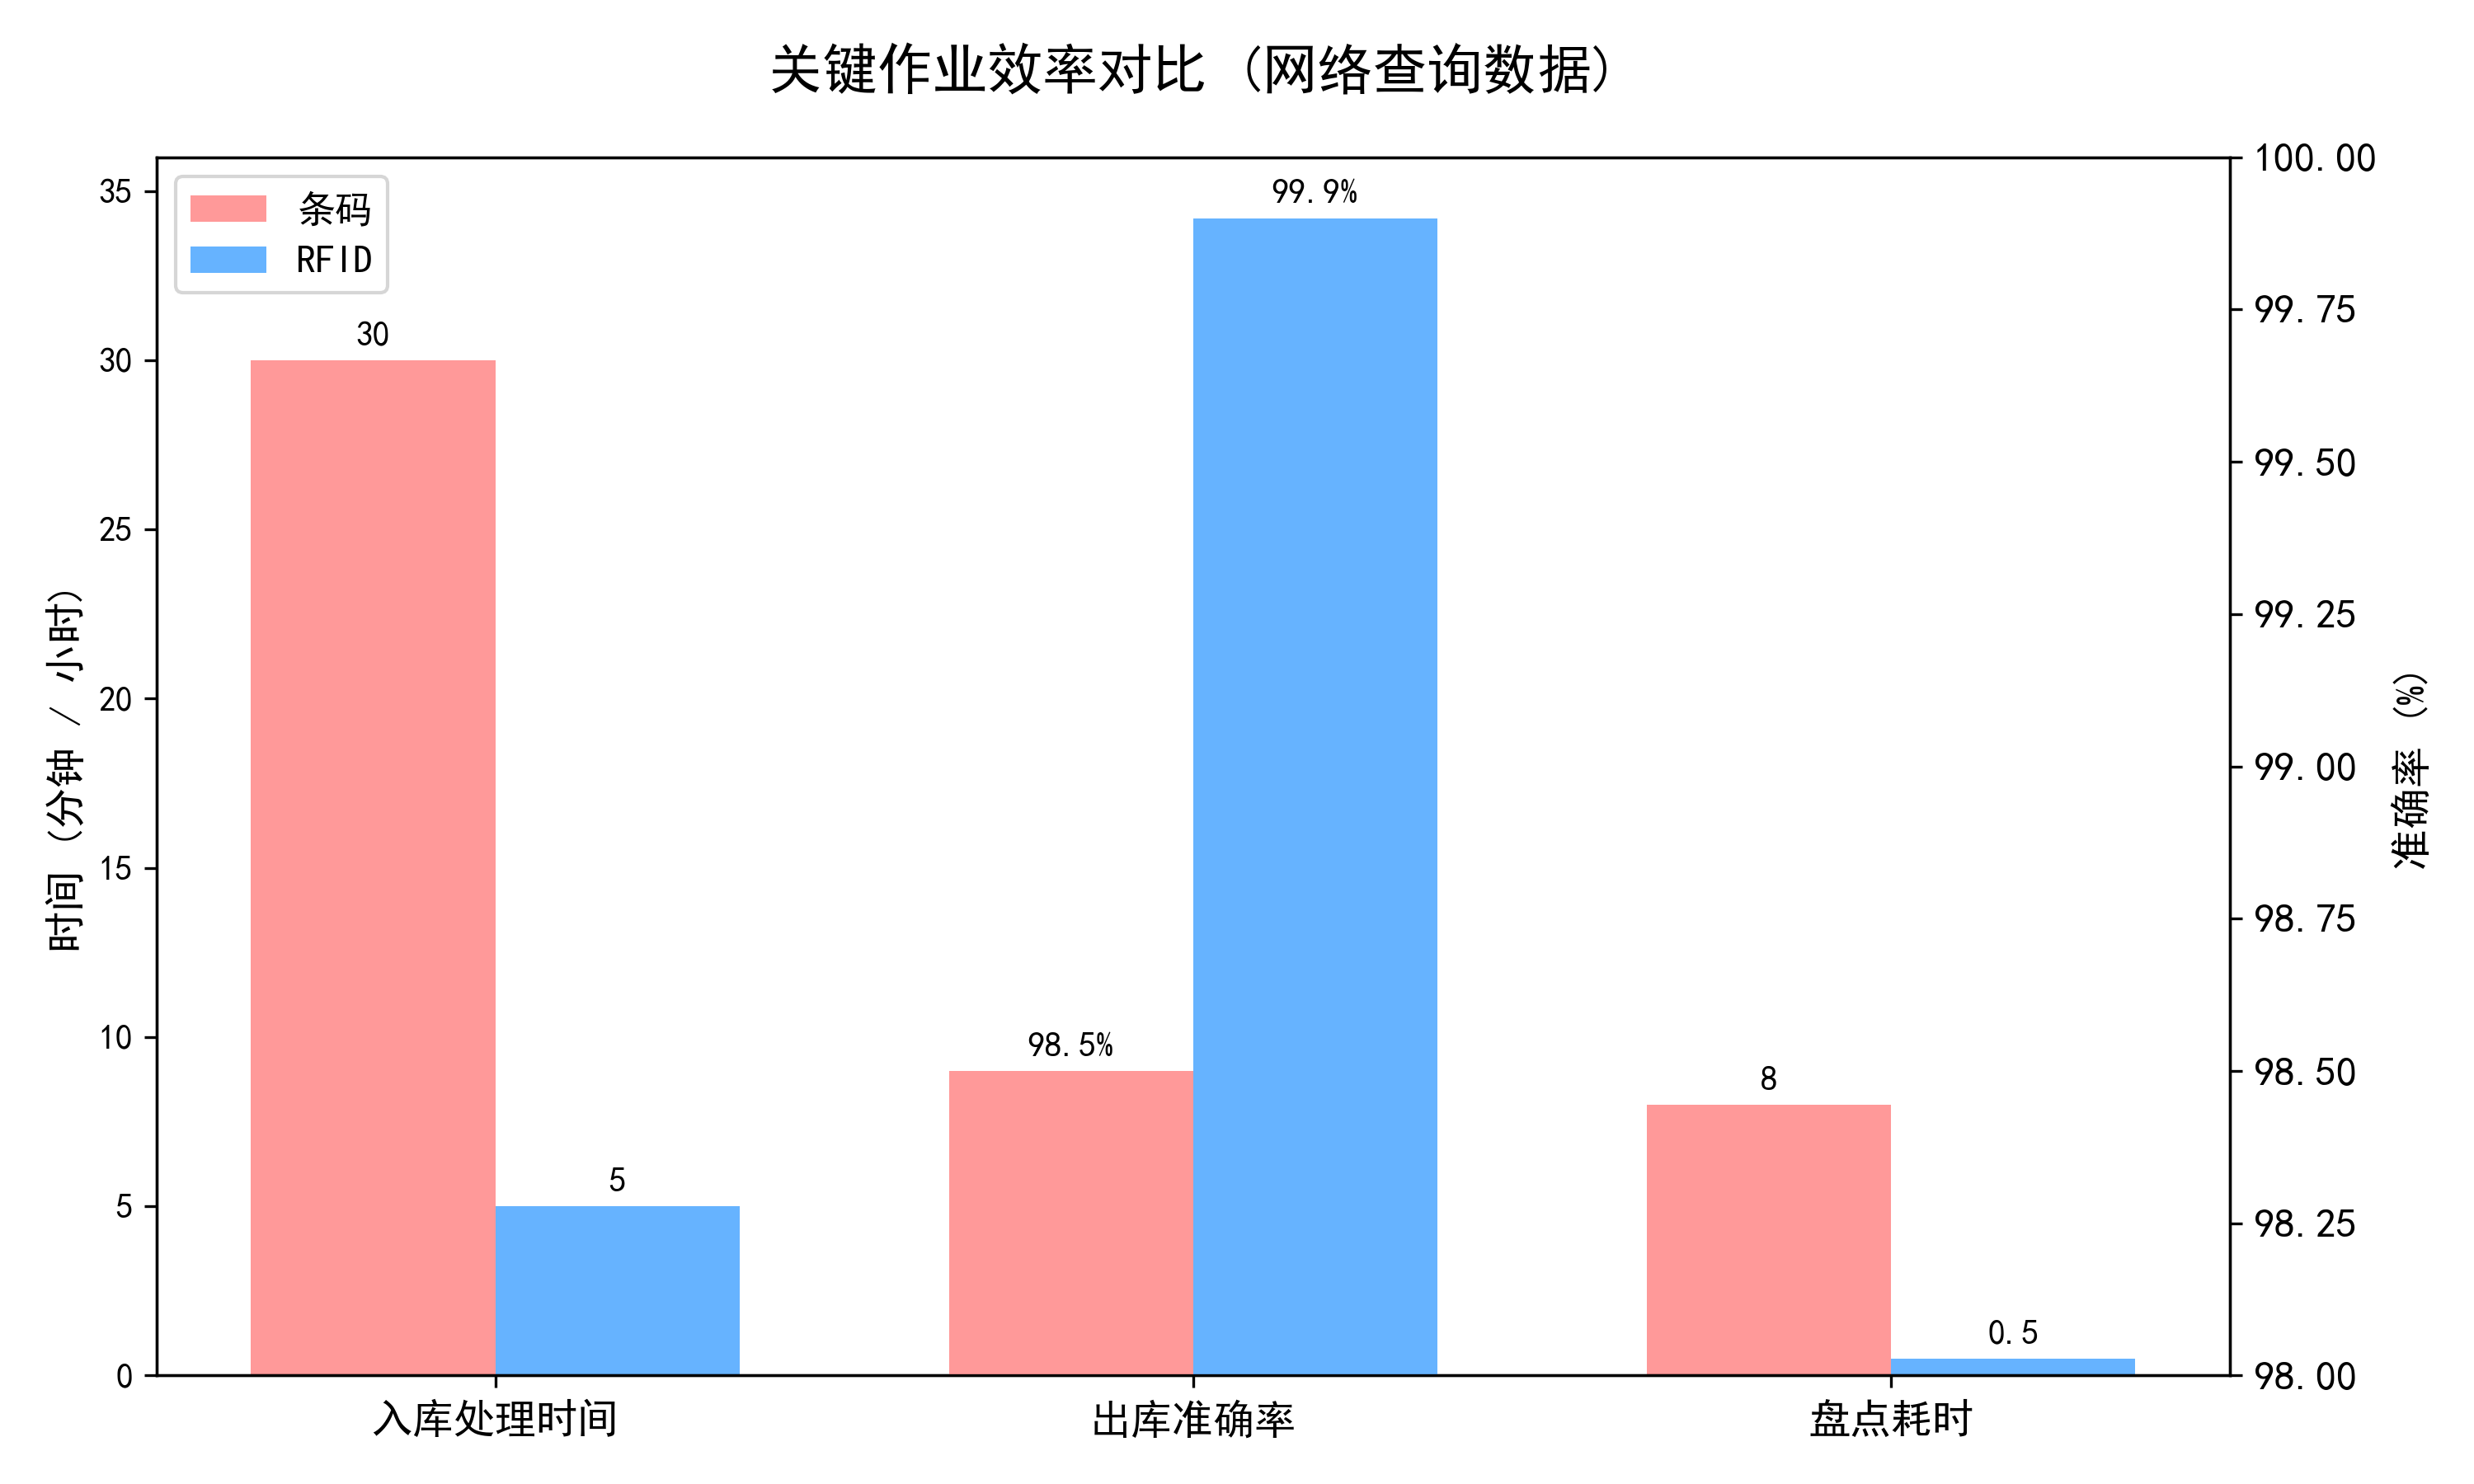
\includegraphics[width=16cm,height=9cm]{efficiency_comparison.png}
    \caption{关键作业效率对比}
    \label{fig:efficiency}
\end{figure}

\subsubsection{技术对比总结}
如 \tablename~\ref{tab:tech_comparison} 所示，RFID技术在多个维度上均优于传统条码技术，体现了其作为智能传感技术在现代物流仓储中的巨大潜力和应用价值。

\begin{table}[H]
    \centering
    \setlength{\belowcaptionskip}{0.3cm} % 调整表格标题与表格的距离
    \caption{RFID技术与传统条码技术对比}
    \label{tab:tech_comparison}
    \begin{tabular}{c c c}
        \toprule
        \textbf{特性} & \textbf{RFID技术} & \textbf{条码技术} \\
        \midrule
        读取方式 & 非接触式，无需对准 & 接触式或近距离，需对准 \\
        同时读取数量 & 可同时读取多个标签 & 一次只能读取一个 \\
        读取距离 & 远（可达数米） & 近（几厘米到几十厘米） \\
        数据容量 & 大（可达KB级别） & 小（几十个字符） \\
        可重复使用性 & 可反复读写 & 一次性印刷，不可更改 \\
        环境穿透性 & 可穿透非金属材料 & 易被遮挡、污损 \\
        成本 & 较高 & 极低 \\
        \bottomrule
    \end{tabular}
\end{table}

\section{结论}

本次实践作业对以RFID读写器为核心的新型智能检测传感器在物料管理领域的应用进行了案例分析。本文通过设定“大型智慧物流中心的自动化物料管理”这一具体场景，深入剖析了该传感技术如何解决传统条码管理模式下入库、出库及盘点效率低下、差错率高等核心问题。

在分析过程中，本文将RFID系统解构为以读写器（传感器）为核心的感知层、被检测目标（电子标签）以及数据处理与应用单元，并详细阐明了其基于射频信号，实现对物料信息进行非接触式、远距离、批量化自动采集的工作原理。

研究结果表明，RFID传感技术的应用，成功地将仓储作业从传统“手动、单点、可视”的数据采集模式，革新为“自动、批量、穿透式”的智能感知模式。这种转变的本质，是利用智能传感器替代了大量重复性的人工作业，从而极大地提升了物料流转效率与数据准确性，为实现仓储精细化、自动化和智能化管理提供了关键的技术支撑。

综上所述，RFID作为一种成熟且强大的智能检测传感技术，在现代物流领域展现出巨大的应用价值和广阔的发展前景。它不仅是解决特定工业场景瓶颈问题的有效工具，更是推动工业4.0和智慧供应链发展的基石技术之一。尽管目前该技术在应用中仍面临成本控制、信号干扰等挑战，但随着技术的持续进步和规模化应用的普及，其必将在构建万物互联的工业物联网（IIoT）体系中扮演愈发重要的角色。

% --- 参考文献部分 ---
\begin{thebibliography}{9}
    \bibitem{ref1} 张言.RFID技术在现代智能物流中的运用[J].无线互联科技,2023,20(10):107-110.DOI:CNKI:SUN:WXHK.0.2023-10-030.
    \bibitem{ref2} 朱心宁,常雯昕,张逸晨,等.基于RFID的溯源和仓储系统研究[J].中国储运,2023,(05):60-61.DOI:10.16301/j.cnki.cn12-1204/f.2023.05.090.
    \bibitem{ref3} 叶秉高,贺静丽.基于RFID电子标签的物联网物流仓储智能定位研究[J].智能物联技术,2025,57(04):169-172.DOI:10.26921/j.cnki.2096-6059.2025.04.036.
    \bibitem{ref4} 李秋玲,臧文轩,孙健,等.RFID技术在文件及货物查找定位中的应用[J].综合运输,2023,45(07):148-153+187.DOI:CNKI:SUN:YSZH.0.2023-07-025.
\end{thebibliography}

\end{document}
% --- 文档结束 ---
